\documentclass{st50_template}
\usepackage{listings}
\usepackage{xcolor}
\usepackage{fancyhdr}
\lstset{language=Matlab}
\begin{document}
\sffamily
\thispagestyle{empty}
\begin{picture}(0,0)
%Images
\put(-90, -122){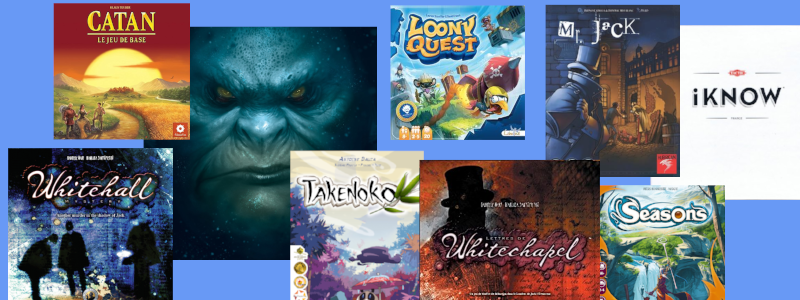
\includegraphics[scale=0.800]{images/banner}}
\put(380, -700){
\includegraphics[scale=0.897]{images/logo_UTBM}}
%Color
\put(-89, -140){\colorbox{black}{\makebox(609, 15){}}}
\put(-89, -226){\colorbox{purple}{\makebox(609, 80){}}}
\put(-89, -247){\colorbox{gray}{\makebox(609, 15){}}}
\put(-89, -633){\colorbox{yellow}{\makebox(609, 380){}}}
%Text
\put(-72, -138){\Large\textcolor{white}{\textbf{UNIVERSITÉ DE TECHNOLOGIE} DE BELFORT-MONTBÉLIARD}}
\put(-72, -193){\Huge\textcolor{white}{Reconnaissance de boîtes de jeux de plateaux}}
\put(-72, -243){\large\textcolor{white}{Rapport de IN52 - IN54}}
\put(-72, -288){\Large{\textbf{BOUCHEREAU Thomas - BRUNET Pierre - PERREZ Stéphane}}}
\put(-62, -308){\large\textcolor{gray}{Département Informatique - Imagerie, Interaction et Réalité Virtuelle}}
%\put(-42, -426){\Large{\textbf{LABORATOIRE SYSTEMES ET TRANSPORTS (IRTES SET)}}}
\put(-62, -408){\large\textcolor{gray}{Université de Technologie de Belfort Montbéliard}}
\put(-62, -423){\large\textcolor{gray}{90 010 - BELFORT CEDEX}}
\put(-72, -568){\large\textcolor{gray}{\textbf{Responsable IN52}}}
\put(-72, -588){\Large{\textbf{Cindy CAPPELLE}}}
\put(320, -568){\large\textcolor{gray}{\textbf{Responsable IN54}}}
\put(320, -588){\Large{\textbf{Yassine RUICHEK}}}
\end{picture}


\fancyhead{}
\cfoot{}

\pagestyle{fancy}
\setlength{\headheight}{20pt} 
\chead{}
\rhead{\thepage}
\renewcommand{\headrulewidth}{0.4pt}
\renewcommand{\footrulewidth}{0.4pt}
\fancyfoot[L]{IN52-54 \quad Bouchereau Thomas - Brunet Pierre - Perrez Stéphane}
\fancyfoot[R]{
\includegraphics[width=2cm]{images/logo_UTBM}}

\definecolor{lightgray}{gray}{0.8}
\newcommand\VRule{\color{lightgray}\vrule width 0.5pt}

\newpage
\thispagestyle{empty}
\tableofcontents

\newpage

\section{Objectifs du projet}

Le but du projet est de faire de la reconnaissance de jeux de plateaux à partir de leur boîte de jeu et d'une base de données. Il nous faut donc procéder en plusieurs étapes. Ainsi, nous devons recentrer la photo sur la face du dessus puis la recadrer afin d'avoir la meilleure analyse possible. Ensuite, nous allons comparer le pourcentage de couleur entre les jeux de la base de données et la photo. Cette base de données est censée se créer au fur et à mesure à l'aide d'une interface.

Nous avons décidé de diviser le projet en trois parties. Ainsi, le premier étudiant s'occuperait du recadrage de la face du dessus de la boîte. Le second prendrait en charge la comparaison de deux images données. Enfin, le dernier créerait la base de données et l'interface graphique afin que l'application soit utilisable en dehors de tests divers.


\section{Développement}

\subsection{Récupérer la face du dessus de la boîte de jeu}
Pour récupérer la face du dessus, il est nécessaire de pouvoir distinguer les contours dans l'image. Nous avons donc décidé d'utiliser la transformée de Hough pour cela. Mais avant tout, il nous faut enlever le bruit de l'image afin d'éviter des contours inutiles. Nous avons donc utiliser la technique d'érosion puis avons rogner l'image en fonction de la densité restante dans les lignes de l'image.

\begin{figure}[ht]
    \centering
    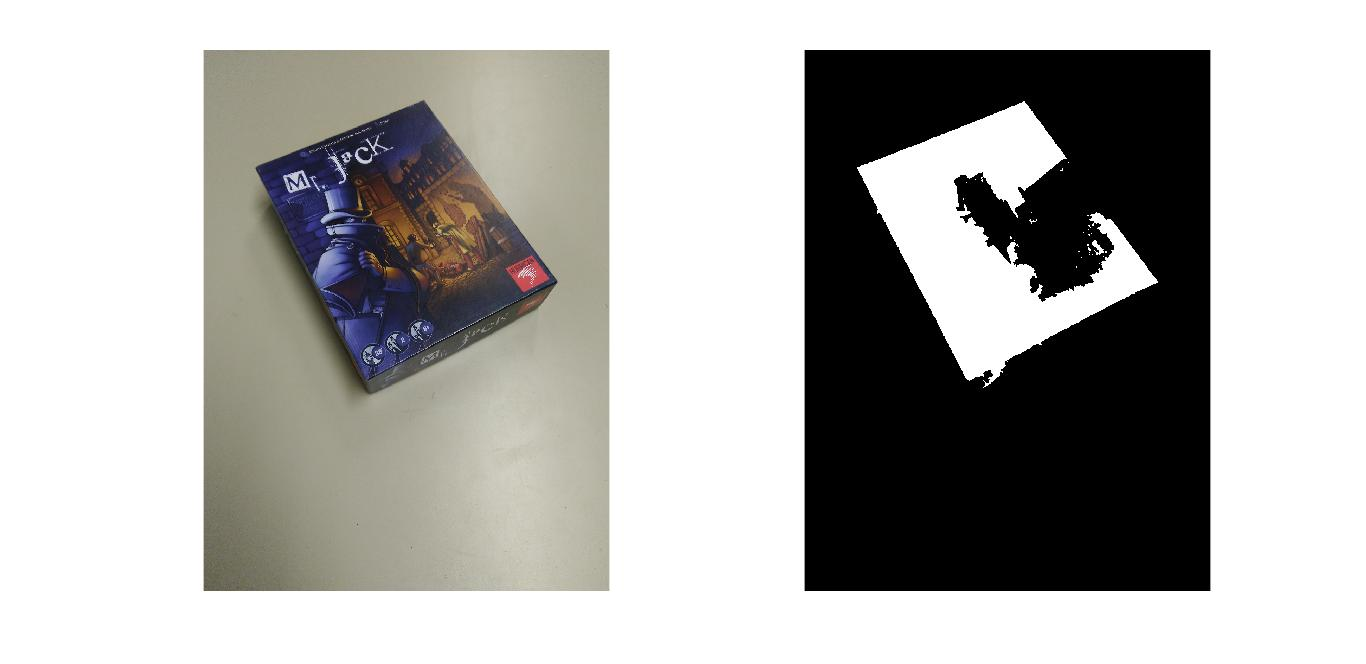
\includegraphics[width=0.77\textwidth]{images/erosion.jpg}
    \caption{Image binaire et érodée}
    \label{erosion}
\end{figure}

\begin{figure}[ht]
    \centering
    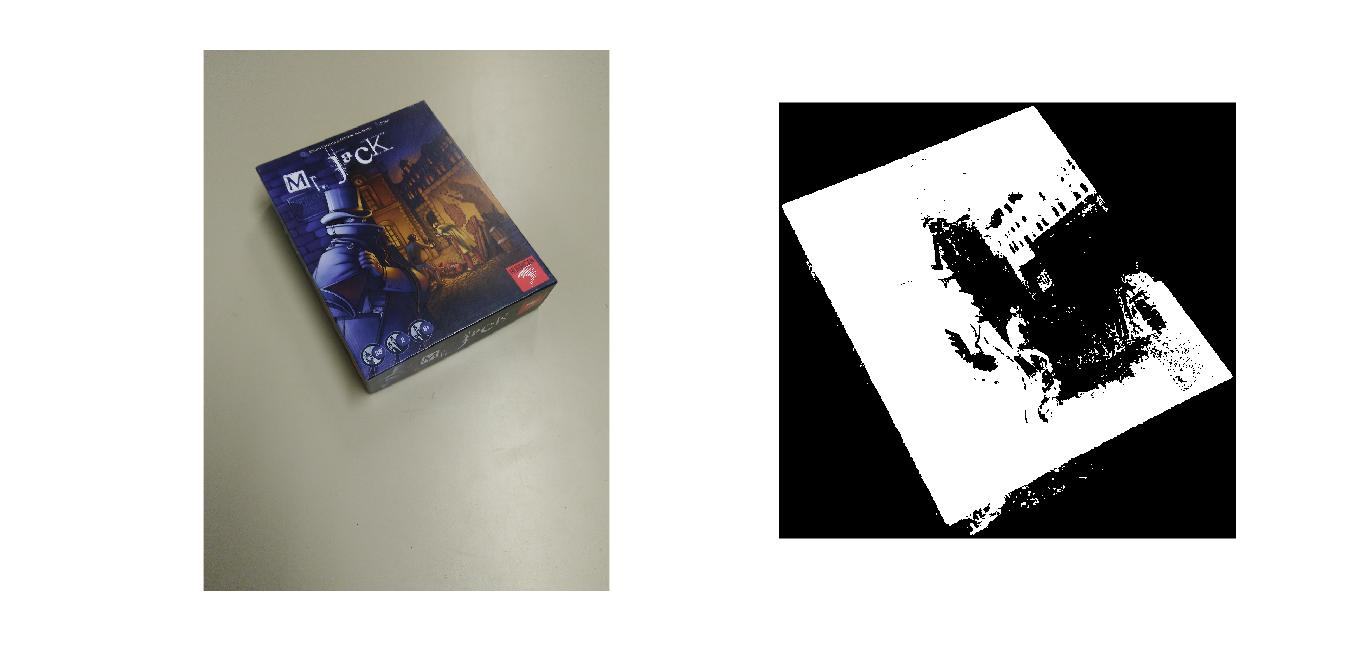
\includegraphics[width=0.77\textwidth]{images/rognage.jpg}
    \caption{Image binaire rognée}
    \label{rognage}
\end{figure}

Après ce pré-traitement, on applique la transformée de Hough à des lignes faisant au moins une certaines longueur pour éviter d'avoir des lignes du dessin du jeu. On allonge ensuite ces lignes et on récupère les points d'intersection. 

Ces points d'intersection ont été produits grâce aux fonctions \emph{polynomes} et \emph{polyval}. Cependant, les lignes générées ne sont pas forcément dans le bon ordre. Par conséquent, les points ne le sont pas non plus. De plus, on génère toutes les intersections de lignes possibles. Il faut donc faire un tri pour éviter les duplicas et également les trier dans un ordre donné. C'est le dernier traitement appliqué avant de passer à l'analyse de l'image.

\begin{figure}[ht]
    \centering
    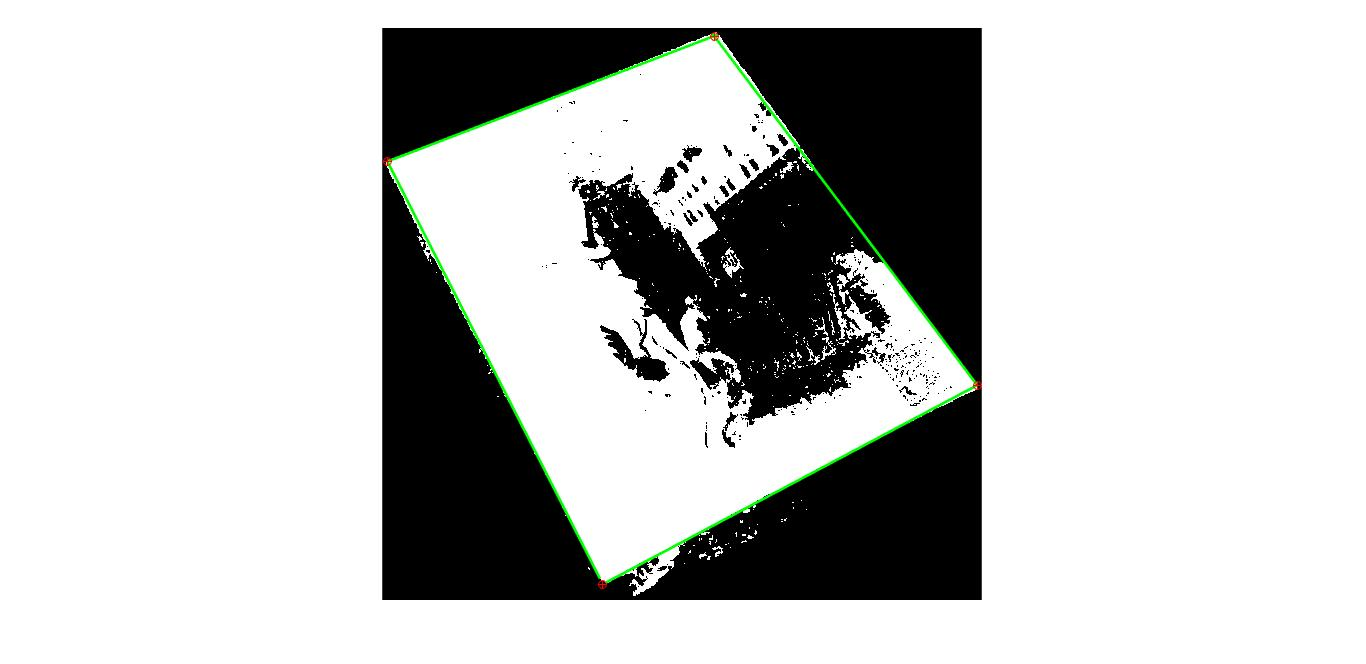
\includegraphics[width=0.77\textwidth]{images/contourEtPts.jpg}
    \caption{Contours de la face du dessus}
    \label{contourEtPts}
\end{figure}

\subsection{De la 3D à la 2D}
Une fois les points récupérés, il nous faut adapter l'image pour la rendre comparable avec l'image de base. On utilise donc les points d'intersection précédemment calculés.

La fonction fitgeotrans permet de rapprocher une image d'une autre grâce à un tableau de points mouvants et un tableau de points fixes. Le tableau de points mouvants doit \emph{rentrer dans} (\emph{fit} en Anglais) le tableau de points fixes.

\begin{figure}[ht]
    \centering
    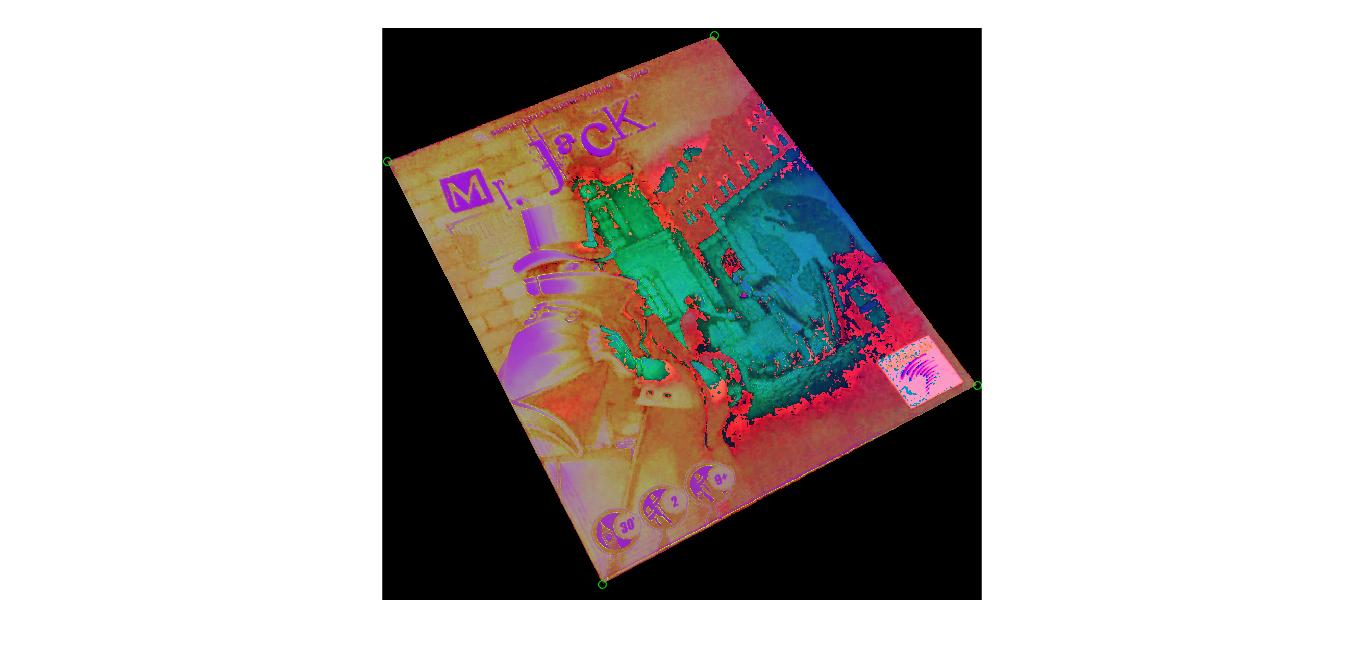
\includegraphics[width=0.77\textwidth]{images/movingPoints.jpg}
    \caption{Points mouvants en vert sur l'image}
    \label{movingPoints}
\end{figure}


C'est à partir de ce moment-là que nous avons rencontré des problèmes. En effet, la fonction n'est pas aussi efficace qu'elle le sous-entend. Malgré tous nos efforts, nous n'avons pu que redresser la boîte sans pouvoir changer les angles de l'image.

Vous verrez sur les figures \ref{geotrans} et \ref{fitgeo} les résultats obtenus grâce à la fonction Matlab fitgeotrans et à un recadrage.

\begin{figure}[ht]
    \centering
    \begin{minipage}[b]{0.45\textwidth}
    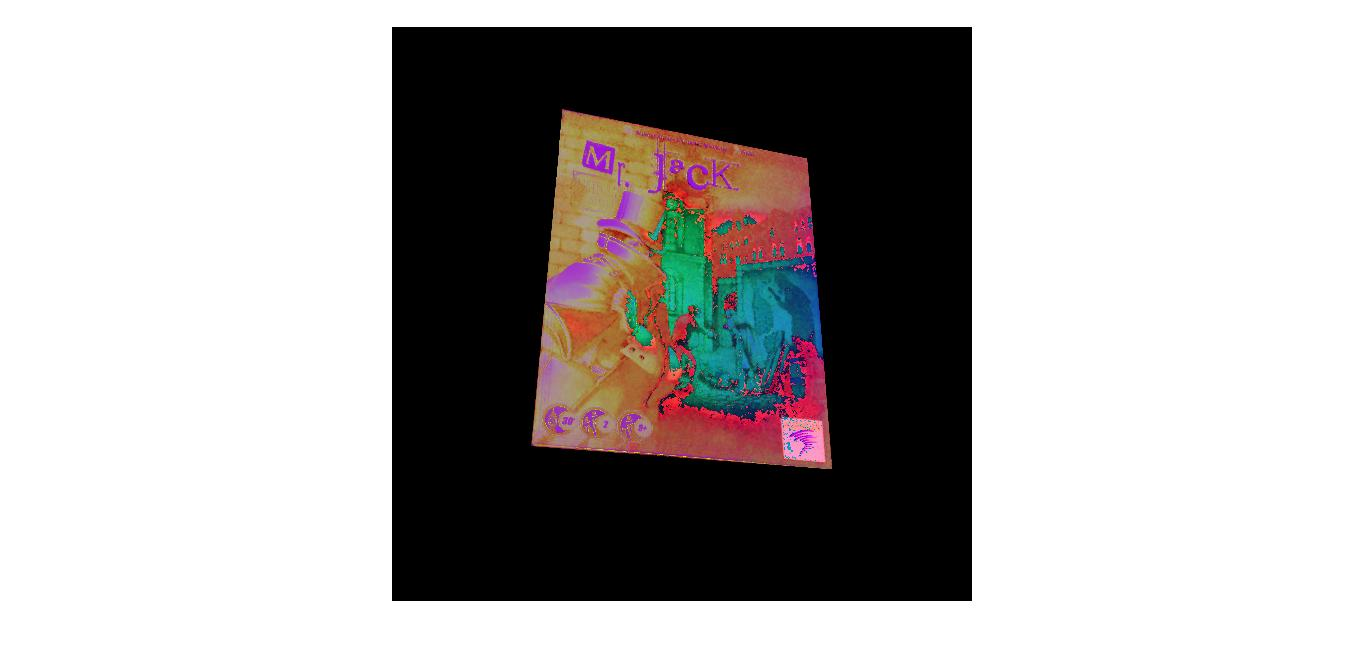
\includegraphics[width=\textwidth]{images/fitgeotrans.jpg}
    \caption{Résultat de la fonction \emph{fitgeotrans}}
    \label{geotrans}
    \end{minipage}
    \hfill
    \begin{minipage}[b]{0.45\textwidth}
    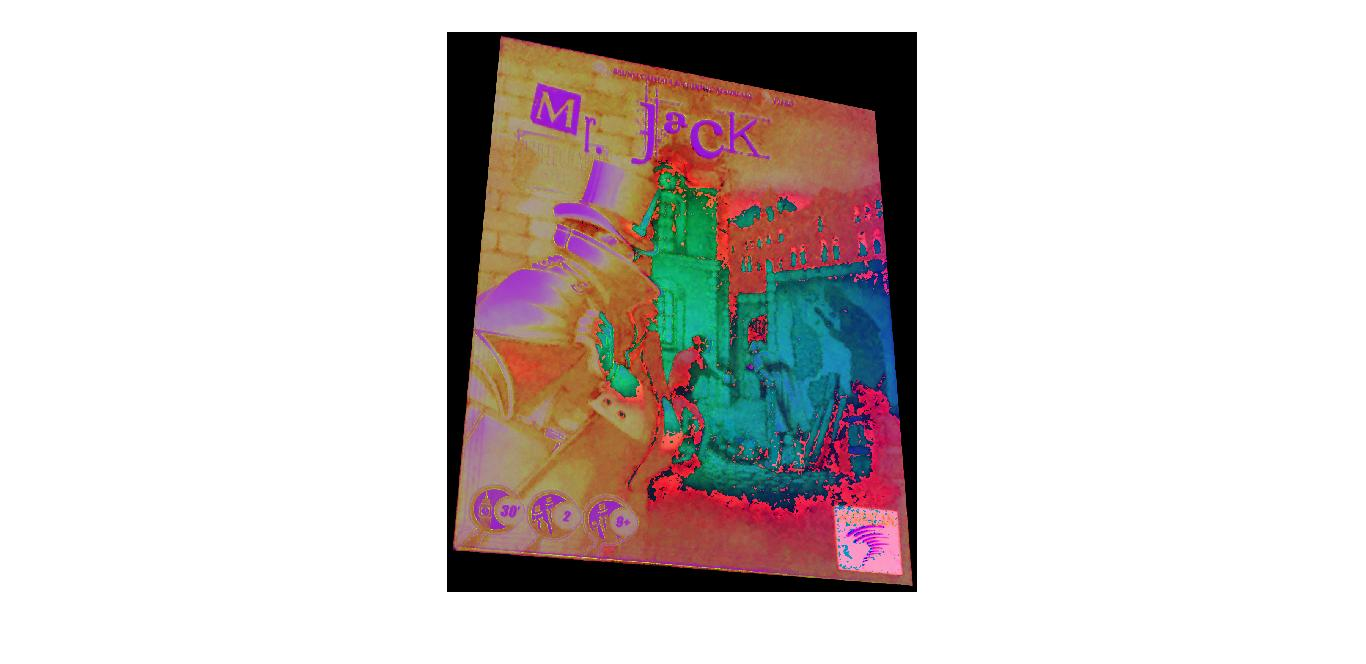
\includegraphics[width=\textwidth]{images/transRecadre.jpg}
    \caption{Recadrage maximal obtenu}
    \label{fitgeo}
    \end{minipage}
\end{figure}

\subsection{Analyse des fréquences}

Nous avons donc décidé de revenir à l'image pré-traitée et ne comparer que les fréquences de couleurs afin de pouvoir rapidement reconnaître un jeu. Cela s'est révélé plus logique et plus optimisé en prenant comme couleurs le HSL. Nous n'avions alors qu'à récupérer le Hue (à savoir la nuance) de chaque pixel et comparer les densités par rapport à la base de données.

Pour savoir quel photo correspond à quel jeu, nous avons récupérer les dessus des boîtes de jeux (trouvés sur des sites marchands) et nous leur avons associé le nom du jeu dans une base de données.

Une fois la photo transformée et recadrée, sans la transformation de \emph{fitgeotrans} pour gagner du temps, nous la comparons avec la base de données.

Voici l'exemple du jeu Loony Quest et de son analyse d'histogramme :

\begin{figure}[ht]
    \centering
    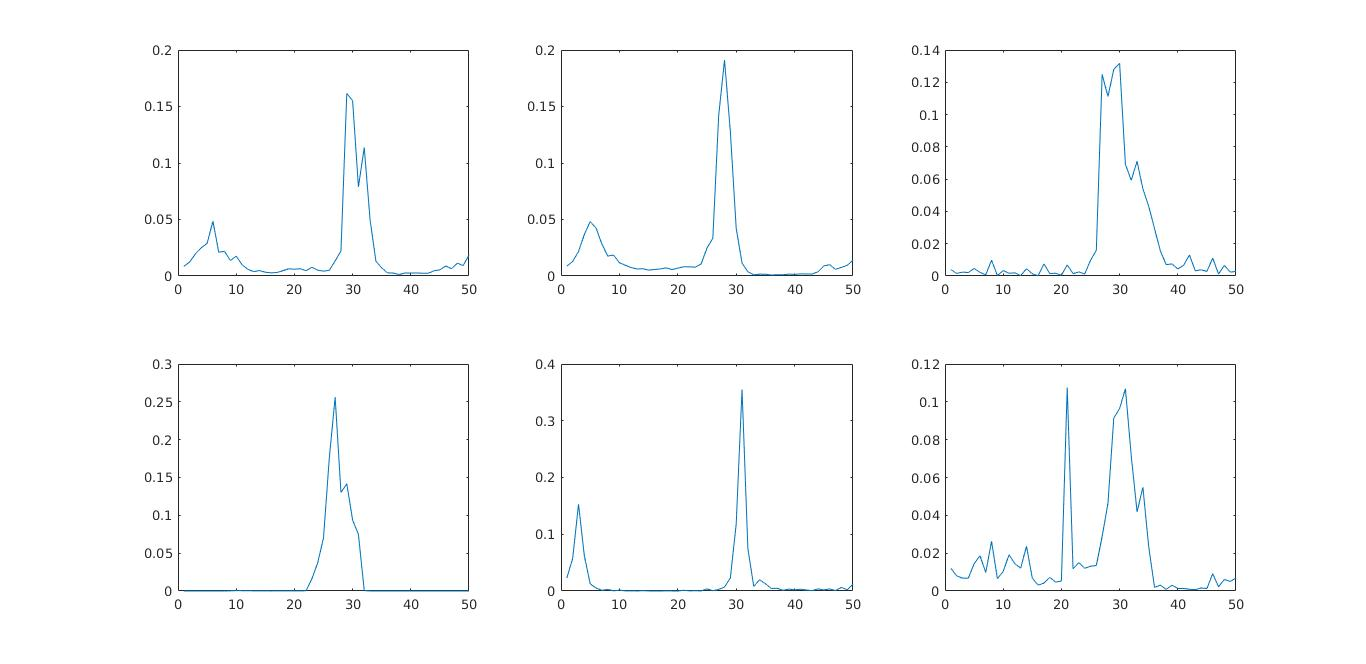
\includegraphics[width=\textwidth]{images/graphLoonyQuest.jpg}
    \caption{Histogrammes de la photo Loony Quest recadrée et des 5 plus proches voisins}
    \label{loonyQuest}
\end{figure}

On voit ainsi que les deux premiers histogrammes sont relativement proches mais peu pratiques à comparer pour un ordinateur. Nous avons donc décidé de créer une fonction calculant la ressemblance entre deux histogrammes. Elle utilise la fonction Matlab \emph{corrcoef} mais avec un delta permettant de décaler la courbe et ainsi vérifier que les couleurs sont proches ou non.

\subsection{Analyse des résultats}

Sur 10 photos de jeux différents testés, 6 fonctionnent sans soucis. Les 10 sont ainsi bien recadrés et analysés mais certains sont peu pratiques à l'analyse. Ainsi, le Takenoko et le IKnow ne fonctionnent pas en raison d'une boîte plus clair que les autres et donc plus sensible au peu de luminosité qu'il y avait lors de la prise de photo.

En revanche, les 6 photos qui fonctionnent ont un pourcentage de ressemblance avoisinant les 90\% pour la plupart. Nous pensons donc que la base de données pourra être complétée à l'avenir et évoluer sur un apprentissage poussé tel que le deep learning.

\subsection{Interface graphique}
Pour permettre à l'utilisateur de facilement utiliser le programme, nous avons mis en place une interface permettant de visualiser le résultat le plus proche ainsi qu'un tableau des cinq meilleures estimations quant à l'identité du jeu.

\begin{figure}[ht]
    \centering
    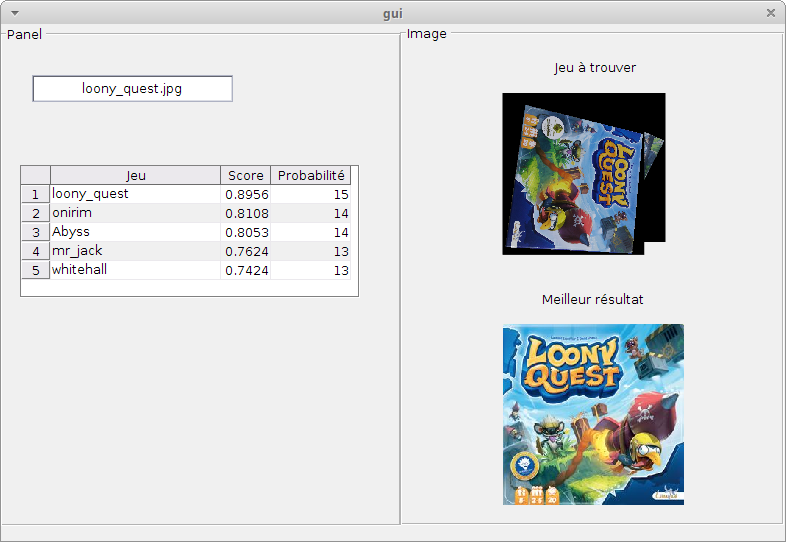
\includegraphics[width=\textwidth]{images/interface.png}
    \caption{Histogrammes de la photo Loony Quest recadrée et des 5 plus proches voisins}
    \label{interface}
\end{figure}

\subsection{Mode d'emploi}
Pour lancer l'application, il suffit de lancer :
\begin{lstlisting}[frame=single]
 $ ./run_gui.sh ''PATH_OF_R2016A_FOLDER''
\end{lstlisting}

Vous pouvez ensuite tester différentes images en mettant le chemin relatif dans le champ de texte demandé et en appuyant sur Entrée. Par exemple, pour l'image de Abyss, il faut préciser ``Images/abyss.jpg''.


\section{Conclusion}

Ce projet a été pour nous très utile et intéressant. En effet, nous nous sommes rendus compte de la difficulté de traitement de photos et nous avons pu tenter plusieurs méthodes afin de retrouver le jeu correspondant. Nous avons ainsi pu utiliser des outils encore peu connus de nous-mêmes sur Matlab. De plus, nous avons appris de nouvelles méthode de comparaison telles que celle du Coefficient de Corrélation utilisée dans notre programme. Enfin, nous avons pu tenter en conditions les éléments appris en cours et en travaux pratiques et dirigés, cela permet d'avoir une expérience réelle de l'imagerie que ce soit dans le traitement comme dans l'analyse d'une image. Nous pensons avoir pu concilier les deux matières dans ce projet.

Dans les améliorations possibles, nous pensons qu'il serait intéressant de combiner plusieurs classifieurs mais également d'intégrer un algorithme de deep-learning. De plus, après avoir utilisé les outils disponibles de Matlab, nous nous demandons s'il ne serait pas plus viable de demander à l'utilisateur de centrer la photo de lui-même. Cela éviterait ainsi du temps de calcul et permettrait d'être encore plus précis dans la comparaison.
\end{document}
